\section{State Rankings}

Using the statistical and (in)distinguishability graph methods described in \cref{sec:stats_methods}, we were able to develop both graph visualizations of state distinguishability and a possible ranking of the states.

\begin{figure}[htb]
    \centering
    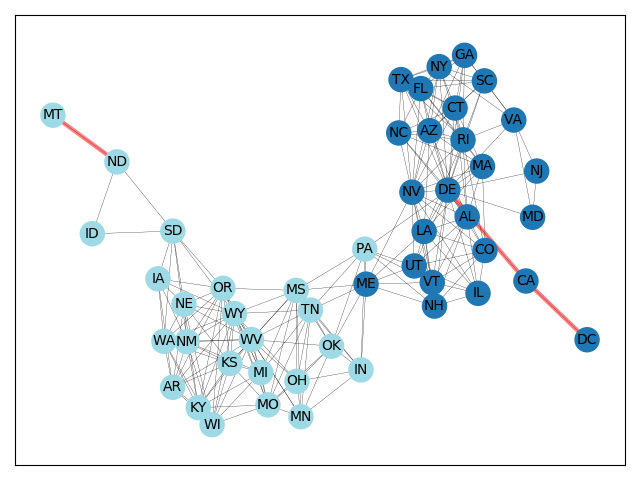
\includegraphics[width=0.65\textwidth]{caida/caida_network_invalid_comps.png}
    \caption{Indistinguishability graph of traceroute data as aggregated by state}
    \label{fig:caida_network_invalid_comps}
\end{figure}

\Cref{fig:caida_network_invalid_comps} shows an indistinguishability graph of comparisons between the states (previously seen in \cref{sec:stats_methods}), where node colors correspond to communities and bold red lines correspond to bridges.\footnote{Bridges can be thought of as indicators of comparison quality; any state on the end of a bridge can be compared to all but one of the other states.} As noted earlier, this graph has no disjoint subgraphs, so ranking by clusters is not possible. \Cref{fig:caida_network_valid_comps} shows the corresponding distinguishability graph, which is much more connected, indicating this data is a good candidate for the topological sort method.

\begin{figure}[htb]
    \centering
    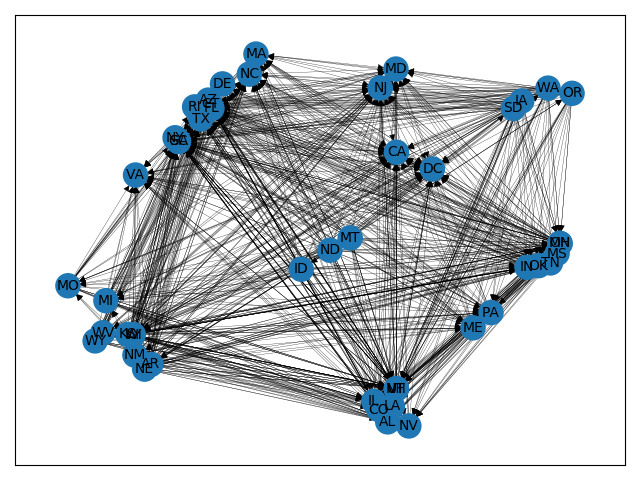
\includegraphics[width=0.65\textwidth]{caida/caida_network_valid_comps.png}
    \caption{Distinguishability graph of traceroute data as aggregated by state}
    \label{fig:caida_network_valid_comps}
\end{figure}

When sorted we obtain a list of 49 states (including the District of Columbia; Hawaii and Alaska were unreachable); two states were not reachable by a maximal topological sort (described in \cref{sec:methods_stats_topological_rankings}). \Cref{tab:caida_topological_state_rankings} shows this ranking, which roughly confirms what we would expect based on prior notions and the heatmaps. Since the topological sort method is based on a graph interpretation and not a traditional sort of means or medians, those values are not shown alongside the states.

\begin{table}[h]
    \centering
    \begin{longtable}{ll|ll|ll|ll|ll}
        \textbf{Rank} & \textbf{State} & \textbf{Rank} & \textbf{State} & \textbf{Rank} & \textbf{State} & \textbf{Rank} & \textbf{State} & \textbf{Rank} & \textbf{State} \\
        \midrule
        \endhead
        \midrule
        \multicolumn{10}{r}{{Continued on next page}} \\
        \endfoot
        \endlastfoot
        \textbf{1 } & DC & \textbf{11} & TX & \textbf{21} &  LA & \textbf{31} & TN & \textbf{41} &    WY \\
        \textbf{2 } & DE & \textbf{12} & AL & \textbf{22} &  NV & \textbf{32} & MN & \textbf{42} &    NE \\
        \textbf{3 } & MD & \textbf{13} & CT & \textbf{23} &  PA & \textbf{33} & OH & \textbf{43} &    NM \\
        \textbf{4 } & CA & \textbf{14} & RI & \textbf{24} &  VT & \textbf{34} & WI & \textbf{44} &    OR \\
        \textbf{5 } & NJ & \textbf{15} & NC & \textbf{25} &  NH & \textbf{35} & KY & \textbf{45} &    IA \\
        \textbf{6 } & NY & \textbf{16} & MA & \textbf{26} &  UT & \textbf{36} & KS & \textbf{46} &    WA \\
        \textbf{7 } & SC & \textbf{17} & AZ & \textbf{27} &  IN & \textbf{37} & MO & \textbf{47} &    ID \\
        \textbf{8 } & GA & \textbf{18} & IL & \textbf{28} &  WV & \textbf{38} & MI & \textbf{48} &    MT \\
        \textbf{9 } & VA & \textbf{19} & CO & \textbf{29} &  MS & \textbf{39} & AR & \textbf{49} &    ND \\
        \textbf{10} & FL & \textbf{20} & ME & \textbf{30} &  OK & \textbf{40} & SD &             &       \\
        \caption{CAIDA+Atlas topologically sorted state rankings}
        \label{tab:caida_topological_state_rankings}
    \end{longtable}
\end{table}

\begin{figure}[htb]
    \centering
    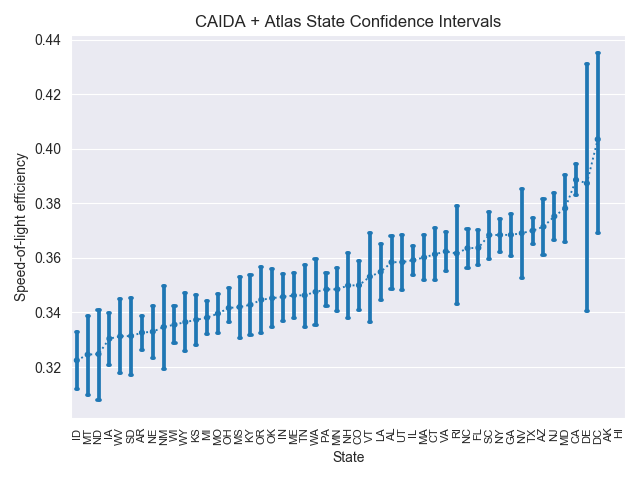
\includegraphics[width=\textwidth]{images/comparative/confidence_intervals/caida_confidence_interval.png}
    \caption{Traceroute confidence intervals for rankings; higher is better}
    \label{fig:caida_confidence_intervals}
\end{figure}

\Cref{fig:caida_confidence_intervals} shows an alternate way of displaying state ranks, using the mean of each state for comparisons. Since data for each state does not follow a normal distribution (see \cref{sec:comparative-distribution} for a variety of \kdes on the subject) the bootstrapping method was used to calculate confidence intervals. Loosely speaking, for each state the "true" mean could be anywhere between the upper and lower bounds of the intervals. \Cref{tab:traceroute_confidence_intervals} shows the specific values for each of these points.

\begin{longtable}{lrrr|lrrr}
\textbf{State} &  \textbf{Min} &  \textbf{Mean} &  \textbf{Max} & \textbf{State} &  \textbf{Min} &  \textbf{Mean} &  \textbf{Max} \\
\midrule
\endhead
\midrule
\multicolumn{8}{r}{{Continued on next page}} \\
\midrule
\endfoot
\endlastfoot

\textbf{DC} &    0.369 & 0.406 &    0.435 & \textbf{WA} &    0.336 & 0.348 &    0.359 \\
\textbf{DE} &    0.342 & 0.390 &    0.432 & \textbf{TN} &    0.335 & 0.347 &    0.357 \\
\textbf{CA} &    0.383 & 0.389 &    0.394 & \textbf{ME} &    0.338 & 0.346 &    0.354 \\
\textbf{MD} &    0.366 & 0.378 &    0.390 & \textbf{IN} &    0.337 & 0.346 &    0.354 \\
\textbf{NJ} &    0.367 & 0.375 &    0.383 & \textbf{OK} &    0.334 & 0.345 &    0.356 \\
\textbf{AZ} &    0.361 & 0.372 &    0.381 & \textbf{OR} &    0.332 & 0.345 &    0.357 \\
\textbf{TX} &    0.365 & 0.370 &    0.375 & \textbf{KY} &    0.332 & 0.343 &    0.354 \\
\textbf{NV} &    0.352 & 0.369 &    0.385 & \textbf{MS} &    0.331 & 0.342 &    0.353 \\
\textbf{GA} &    0.361 & 0.369 &    0.376 & \textbf{OH} &    0.334 & 0.342 &    0.349 \\
\textbf{NY} &    0.363 & 0.369 &    0.375 & \textbf{MO} &    0.332 & 0.340 &    0.347 \\
\textbf{SC} &    0.359 & 0.369 &    0.377 & \textbf{MI} &    0.332 & 0.338 &    0.344 \\
\textbf{FL} &    0.357 & 0.364 &    0.370 & \textbf{KS} &    0.328 & 0.337 &    0.347 \\
\textbf{NC} &    0.356 & 0.364 &    0.370 & \textbf{WY} &    0.326 & 0.337 &    0.347 \\
\textbf{RI} &    0.343 & 0.363 &    0.379 & \textbf{WI} &    0.329 & 0.336 &    0.342 \\
\textbf{VA} &    0.355 & 0.362 &    0.369 & \textbf{NM} &    0.320 & 0.335 &    0.350 \\
\textbf{CT} &    0.352 & 0.361 &    0.371 & \textbf{NE} &    0.324 & 0.333 &    0.343 \\
\textbf{MA} &    0.352 & 0.360 &    0.368 & \textbf{AR} &    0.326 & 0.333 &    0.339 \\
\textbf{IL} &    0.354 & 0.359 &    0.364 & \textbf{SD} &    0.317 & 0.332 &    0.346 \\
\textbf{UT} &    0.348 & 0.359 &    0.369 & \textbf{WV} &    0.318 & 0.331 &    0.345 \\
\textbf{AL} &    0.349 & 0.359 &    0.368 & \textbf{IA} &    0.321 & 0.331 &    0.340 \\
\textbf{LA} &    0.345 & 0.355 &    0.365 & \textbf{ND} &    0.308 & 0.326 &    0.341 \\
\textbf{VT} &    0.337 & 0.354 &    0.369 & \textbf{MT} &    0.310 & 0.325 &    0.339 \\
\textbf{CO} &    0.341 & 0.350 &    0.359 & \textbf{ID} &    0.312 & 0.322 &    0.333 \\
\textbf{NH} &    0.338 & 0.350 &    0.362 & \textbf{AK} &          &       &          \\
\textbf{MN} &    0.340 & 0.349 &    0.356 & \textbf{HI} &          &       &          \\
\textbf{PA} &    0.342 & 0.349 &    0.355 &             &          &       & \\
\caption{Traceroute state confidence intervals}
\label{tab:traceroute_confidence_intervals}
\end{longtable}


The confidence intervals for each state's mean are large, indicating that there are few meaningful comparisons to be made here. The same conclusion can be drawn from the indistinguishability graph in \cref{fig:caida_network_invalid_comps}; there are no disjoint subgraphs so a ranking by groups of states cannot even be drawn. The topological sorting results shown in \cref{tab:caida_topological_state_rankings} are interesting but they have the fundamental flaw of topological sorts as described in \cref{sec:methods_stats_topological_rankings}: the sorting relies on implicit comparisons that cannot be made according to this data set.

The underlying problem is not with variance in the data itself (as shown by \cref{fig:caida_cv_distribution} and \cref{fig:caida_stdev_distribution} the data spread is low, proving quality data), but in the aggregation method. As visualized in \cref{fig:caida_idw_heatmap} there is simply too much variation within a state, prohibiting a statistically-valid ranking of all 50 of them. We can make simple assertions where confidence intervals do not overlap, or between two states where $p<0.05$, but unfortunately nothing beyond that.

The conclusions that we \textit{can} draw on a state level are that, loosely speaking, states that are more populated or more urban tend to have better internet than those are are less populated or more rural on average. The District of Columbia, being only a city and also the seat of the \us federal government, has the best internet. On the other hand, sparsely populated states like Montana or North Dakota rank at absolute last. To get an accurate idea of internet connectivity, the only statistically-valid choice is to use aggregation by a narrower area, or a continuous interpolation method like the \idw heatmap in \cref{fig:caida_idw_heatmap}.
